\documentclass[12pt]{article}
\usepackage{amsmath} % AMS Math Package
\usepackage{bm}
\usepackage{amsthm} % Theorem Formatting
\usepackage{amssymb}    % Math symbols such as \mathbb
\usepackage{graphicx} % Allows for eps images
\usepackage[dvips,letterpaper,margin=1in,bottom=0.7in]{geometry}
\usepackage{tensor}
\usepackage{amsmath}
\usepackage{siunitx}
\usepackage{physics}
\usepackage{amsmath, amssymb, graphics, setspace}

\newcommand{\mathsym}[1]{{}}
\newcommand{\unicode}[1]{{}}

\newcounter{mathematicapage}

\newtheorem{p}{Problem}
\usepackage{cancel}
\newtheorem*{lem}{Lemma}
\theoremstyle{definition}
\newtheorem*{dfn}{Definition}
 \newenvironment{s}{%\small%
        \begin{trivlist} \item \textbf{Solution}. }{%
            \hspace*{\fill} $\blacksquare$\end{trivlist}}%

\makeatletter
% we use \prefix@<level> only if it is defined
\renewcommand{\@seccntformat}[1]{%
  \ifcsname prefix@#1\endcsname
    \csname prefix@#1\endcsname
  \else
    \csname the#1\endcsname\quad
  \fi}
% define \prefix@section
\newcommand\prefix@section{}
\newcommand{\prefix@subsection}{}
\newcommand{\prefix@subsubsection}{\thesubsubsection\ - }
\renewcommand{\thesubsection}{\arabic{subsection}}
\makeatother

\begin{document}

 {\noindent\Huge\bf  \\[0.5\baselineskip] {\fontfamily{cmr}\selectfont  Project 1}         }\\[2\baselineskip] % Title
{ {\bf \fontfamily{cmr}\selectfont Quantum Mechanics}\\ {\textit{\fontfamily{cmr}\selectfont     \today}}}~~~~~~~~~~~~~~~~~~~~~~~~~~~~~~~~~~~~~~~~~~~~~~~~~~~~~~~~~~~~~~~~~~~~~~~~~~~~~    {\large \textsc{C Seitz}
\\[1.4\baselineskip] 

\section{Part 1}

\textbf{(A)} We were given the Hamiltonian:

\begin{equation*}
-t(\phi_{n,i+1} + \phi_{n,i-1}) + (2t+V_{i})\phi_{n,i} = \epsilon_{n}\phi_{n,i}
\end{equation*}

which gives us a relationship between $\phi_{n,i}$ and the neighboring elements $\phi_{n,i-1}$ and $\phi_{n,i+1}$. The explicit matrix form is

\begin{equation}
\hat{H}_{0}\phi_{n} = \begin{pmatrix}
2t + V_{1} & -t & 0 & \hdots\\
-t & 2t + V_{2} & -t& \hdots\\
0 & -t & 2t + V_{3}& \hdots\\
\vdots & \vdots & \vdots & \ddots
\end{pmatrix}
\begin{pmatrix}
\phi_{n,1}\\
\phi_{n,2}\\
\phi_{n,3}\\
\vdots
\end{pmatrix} = \epsilon_{n}\begin{pmatrix}
\phi_{n,1}\\
\phi_{n,2}\\
\phi_{n,3}\\
\vdots
\end{pmatrix}
\end{equation}

The full matrix $\hat{H}_{0}$ is shown in Figure 1a. 
\vspace{0.1in}\\
\noindent \textbf{(B)} From (1) we can see that the diagonal elements represent the discretized potential $V_{n}$ (plus a constant $2t$ where $t = \frac{\hbar^{2}}{2ma^{2}}$). The off-diagonal elements are just constants with dimension of energy over length squared. The matrix of normalized eigenvectors of $\hat{H}_{0}$ are shown in Figure 1b.
\vspace{0.1in}\\
\noindent\textbf{(C)} To show that the eigenvectors form an orthonormal set, We can define a matrix $T$ such that each column of $T$ is one eigenvector $\vec{\phi}_{n}$ of $\hat{H}_{0}$. If the eigenvectors are indeed orthonormal, then

\begin{equation*}
T^{T}T = I
\end{equation*}

This product is shown in Figure 1c, and we can see that the eigenvectors are orthonormal.

\begin{figure}[t!]
\centering
\includegraphics[width=15cm]{Figure_1}
\caption{(A) The Hamiltonian $H_{0}$ (B) Eigenvectors as columns of a matrix (sorted by ascending eigenvalue) (C) Eigenvalue spectrum sorted in ascending order}
\label{fig:method}
\end{figure}

\vspace{0.1in}
\noindent \textbf{(D)} The sorted eigenvalues are shown in Figure 1d.

\vspace{0.1in}
\noindent \textbf{(E)} Three example probability distributions are shown in Figure 2



\vspace{0.1in}
\noindent \textbf{(F)} The standard quantum mechanics problem this corresponds to is the free particle.

\begin{equation*}
-\frac{\hbar^{2}}{2m}\frac{\partial^{2}\psi}{\partial x^{2}} = E\psi
\end{equation*}

\begin{equation*}
\frac{\partial^{2}\psi}{\partial x^{2}} = -k^{2}\psi
\end{equation*}

for $k = \frac{\sqrt{2mE}}{\hbar}$. So clearly the energy eigenvalues are $E_{k} = \hbar k^{2}/2m$. Notice that $k$ is a continuous parameter and therefore there is a continuum of solutions to the eigenvalue equation. The general solution to the above equation is

\begin{equation*}
\psi(x) = Ae^{ikx}
\end{equation*}

We would expect that the energy eigenvalues in Figure 1d would vary quadratically in $n$; however, the curve has a more sigmoidal shape. Around $n=50$, we can see that the eigenvalues are increasing more linearly because those solutions are actually superpositions of harmonics (See Figure 2, $n=50$ in purple). 

\begin{figure}[t!]
\centering
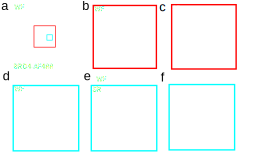
\includegraphics[width=10cm]{Figure_2}
\caption{Energy eigenkets in the position representation for $n=0,10,50$}
\label{fig:method}
\end{figure}

\vspace{0.1in}
\noindent \textbf{(G)} To understand why there are beats (for example see $n=50$), notice that another perfectly valid solution of Schrodinger's equation is


\begin{align*}
\psi(x) &= Ae^{ikx} + Be^{ik'x} \\
&= e^{i(k+k')x/2}\left(Ae^{i(k-k')x/2)} + Be^{-i(k-k')x/2}\right)
\end{align*}

which is a wave with frequency $k-k'$ modulated by the average frequency $(k+k')/2$. 
Furthermore, eigenvalue curve plateaus as $n\rightarrow 100$ because we have chosen a finite sampling frequency $a$, and higher energy solutions cannot be resolved.

\vspace{0.1in}
\noindent \textbf{(H)} The unitary operator that transforms $\hat{H_{0}}$ into the $\ket{n}$ basis to the $\ket{\phi_{n}}$ basis is simply

\begin{align*}
U_{0} = T^{-1}
\end{align*}

which we can use to represent our Hamiltonian in the energy basis (we are just diagonalizing the Hamiltonian)

\begin{align*}
\hat{H} = U_{0} H_{0} U_{0}^{-1}
\end{align*}

$\hat{H}$ is shown in Figure 3a, and is diagonal.

\vspace{0.1in}
\noindent \textbf{(I)} The values along the diagonal of $\hat{H}$ are the energy eigenvalues

\vspace{0.1in}
\noindent \textbf{(J)} The energy eigenvalues are shown in Figure 3b

\vspace{0.1in}
\noindent \textbf{(K)} The energy eigenvalues are the same as they were before the change of basis. All we have done is changed our representation, so they should be. 

\vspace{0.1in}
\noindent \textbf{(L)} Three representative probability distributions are shown in Figure 3d. These are delta functions because we have changed to the energy basis.

\begin{figure}[t!]
\centering
\includegraphics[width=15cm]{Figure_3}
\caption{(A) The Hamiltonian $H_{0}$ after unitary transformation with $U_{0}$ (B) Eigenvalue spectrum sorted in ascending order (C) Eigenvectors as columns of a matrix (sorted by ascending eigenvalue) (D) Probability densities for a few eigenvectors in the energy basis}
\label{fig:method}
\end{figure}

\section{Part 2}

\vspace{0.1in}
\noindent \textbf{(M)} The Hamiltonian matrix is shown in Figure 4a.

\vspace{0.1in}
\noindent \textbf{(N)} $\hat{H}$ differs from $\hat{H}_{0}$ from zero to the 29th element and the 69th element to the 100th element along the diagonal. This is because we have set $V=V_{L}$ for $0 \leq x \leq 29a$ and $V=V_{R}$ for $69a\leq x \leq 100$. The matrix $\hat{H}$ is shown in Figure 1a, its sorted eigenvectors are shown in Figure 4b, and their corresponding eigenvalues, sorted in ascending order, are shown in Figure 4d. 

\begin{figure}[t!]
\centering
\includegraphics[width=15cm]{Figure_4}
\caption{(A) The Hamiltonain $H$ (B) Eigenvalue spectrum sorted in ascending order (C) Eigenvectors as columns of a matrix (sorted by ascending eigenvalue)}
\label{fig:method}
\end{figure}

\vspace{0.1in}
\noindent \textbf{(O)} The energy eigenvalues for this Hamiltonian are shown in Figure 4d.

\vspace{0.1in}
\noindent \textbf{(P)} Probability distributions for $n=1, 25, 26, 35, 39, 41, 55$ are shown in Figure 5.

\vspace{0.1in}
\noindent \textbf{(Q)} For $n=0$ a particle is most likely to be in the region where $V=0$, which makes sense because this is the ground state. As we increase the energy for $n=24,25,34$, we see that the particle is no longer bound to the potential well ($E > V_{L}$), but it doesn't have enough energy to be found from $69a\leq x \leq 100$ where $V=V_{R}$ (($E < V_{R}$). So we see decaying exponenitals there. Furthermore, for $n=38,40,54,55$ we see sinusoidal solutions in both regions $0 \leq x \leq 29a$ and $69a\leq x \leq 100$. Clearly the energy is then high enough for the particle to be found there ($E > V_{R}$).

\vspace{0.1in}
\noindent \textbf{(R)} There are kinks in the energy eigenvalue plot because neighboring eigenvectors have more similar energy eigenvalues than before. Presumably this is because the asymmetric shape of the promotes a more discontinuous eigenvalue spectrum.

\vspace{0.1in}
\noindent \textbf{(S)} The matrix after unitary transformation is shown in Figure 6a.

\vspace{0.1in}
\noindent \textbf{(T)} 

\begin{figure}[t!]
\centering
\includegraphics[width=17cm]{Figure_5}
\caption{Probability densities for a few eigenkets of $H$}
\label{fig:method}
\end{figure}
\vspace{0.1in}
\noindent \textbf{(U)} The eigenvalue plot for $U_{0}H U_{0}^{-1}$ is the same as for $H$, as they should be. Again, we have changed our representation but nothing physical has changed.

\vspace{0.1in}
\noindent \textbf{(V)} The probability distributions $|\bra{\phi_{0,m}}\ket{\phi_{n}}|^{2}$ for $n=1, 25, 26, 35, 39, 41, 55$ are shown in Figure 7.

\vspace{0.1in}
\noindent \textbf{(W)} Let $\ket{\phi_{n}}$ be an orthonormal set of energy eigenkets of $\hat{H}$ and $\ket{\phi_{m}}$ be an orthonormal set of eigenkets of $\hat{H_{0}}$. Then $\sum_{m}\ket{\phi_{m}}\bra{\phi_{m}}\ket{\phi_{n}}$ is the representation of $\ket{\phi_{n}}$ in the $\ket{\phi_{m}}$ basis. It follows that $|\bra{\phi_{m}}\ket{\phi_{n}}|^{2}$ is the norm squared of that representation. Ultimately, we see spikes because for certain $m$, because $\bra{\phi_{n}}\ket{\phi_{n}}$ has greater magnitude.

\vspace{0.1in}
\noindent \textbf{(X)} The matrix of values $\bra{\phi_{m}}\ket{\phi_{n}}$ is shown in Figure 6c. Each column of this matrix is an eigenvector $\ket{\phi_{n}}$ in the $\ket{\phi_{m}}$ basis. We can see that the kets $\ket{\phi_{n}}$ are superpositions of the plane wave solutions to the free particle problem. This makes sense, because using Fourier analysis, we should be able to construct arbitrary wavefunctions using a basis consisting of fundamental harmonics.


\begin{figure}[t!]
\centering
\includegraphics[width=16cm]{Figure_6}
\caption{(A) The Hamiltonain after unitary transformation with $U_{0}$ (B) Eigenvalue spectrum sorted in ascending order (C) Eigenvectors as columns of a matrix (sorted by ascending eigenvalue)}
\label{fig:method}
\end{figure}

\begin{figure}[t!]
\centering
\includegraphics[width=17cm]{Figure_7}
\caption{Representative probability distributions for eigenvectors of $H$ in $H_{0}$ eigenbasis}
\label{fig:method}
\end{figure}

\end{document}